% Zurich Tree Management — research paper
% Build: pdflatex zurich-tree-management.tex (twice). Figures in figures/.

\documentclass[11pt,a4paper]{article}
\usepackage[utf8]{inputenc}
\usepackage[T1]{fontenc}
\usepackage{lmodern}
\usepackage{microtype}
\usepackage[margin=2.5cm]{geometry}
\usepackage{booktabs}
\usepackage{array}
\usepackage{parskip}
\usepackage{enumitem}
\usepackage{graphicx}
\usepackage{subcaption}
\usepackage{xcolor}
\usepackage{tikz}
\usetikzlibrary{arrows.meta,positioning,fit,backgrounds}
\usepackage[hidelinks]{hyperref}
\usepackage{url}

\linespread{1.08}
\graphicspath{{figures/}}
\setlist{itemsep=2pt,topsep=4pt}

\newcommand{\appname}{Zurich Tree Management}
\newcommand{\repourl}{https://github.com/suadarzimanli/zurich-tree-management}
\newcommand{\archivedoi}{(DOI assigned on archiving)}

\title{Anchoring Urban Tree Service Requests to the Tree:\\
       A Design Study and City-Wide Location Analysis\\ Using Zürich Open Data}
\author{Suad Arzimanli\\[2pt]
        \small University of \L{}ód\'{z}, Faculty of Mathematics and Computer Science, Poland\\
        \small \texttt{suad.arzimanli@gmail.com}}
\date{}

\begin{document}
\maketitle

\begin{abstract}
Residents report fallen branches, hazardous limbs and planting requests to municipal tree departments, usually by describing a location in words. Staff then work each case through inspection and field work across separate maps, lists and records. This paper presents a design study of an alternative organisation: every report is \emph{anchored to one tree} from the city's open tree cadastre and remains \emph{one service request (SR)} from intake to closure, with a public status view that never reveals who filed it. I describe the case model, the design principles drawn from civic-reporting and case-management practice, and an open-source demonstrator built on the City of Zürich \emph{Baumkataster}.

The central empirical question is how much location ambiguity tree-anchored intake removes. Using all 81{,}403 trees in the cadastre and all 59{,}330 official building addresses, I count the candidate trees a report leaves for staff to disambiguate. For street trees, a building address leaves a median of three candidates and identifies a single tree in only 14\% of cases; for park trees, 3\%, and 15\% of all trees are more than 60\,m from any address. A simulation of imprecise touch input then compares four map-selection rules. Offering every tree within 10\,m, ordered by distance, keeps the intended tree among the choices in at least 99.8\% of street-tree taps with errors up to 8\,m and never attaches a report to the wrong tree silently, at the cost of one confirming tap on a short list (median two trees). Selecting the nearest tree automatically is faster but attaches the wrong tree in 26\% of street-tree taps at a 5\,m error. The results support tree-anchored intake with an explicit confirmation step, and show that the selection radius must be set against realistic touch error.

\medskip
\noindent\textbf{Keywords:} urban forestry; service requests; open government data; asset-based reporting; location ambiguity; web GIS; privacy by design; design science.

\smallskip
\noindent\textbf{Disclaimer.} The \appname{} application is an independent academic demonstrator. It is not affiliated with, endorsed by or operated on behalf of the City of Zürich.
\end{abstract}

%======================================================================
\section{Introduction}
\label{sec:intro}

Urban trees provide shade, improve air quality and shape the character of neighbourhoods \cite{beatley2011,escobedo2011}. When something goes wrong---a hanging branch over a footpath, a tree blocking a road after a storm, a missing tree in a row---residents contact the city. Each contact becomes a \emph{service request}: a location, a category and a lifecycle that may include an inspection by an arborist and work by a crew or contractor.

Two weaknesses recur in how such requests are handled. First, \emph{location}: residents describe where the problem is, typically with an address or a street name, and staff must later decide which tree is meant. Second, \emph{continuity}: intake, inspection and field work are often recorded in separate modules with their own identifiers, so the story of a case is hard to follow and hard to report back to the resident.

Cities now publish tree inventories as open data \cite{janssen2012}. Zürich's \emph{Baumkataster} lists the trees managed by the city, each with a unique tree number, species, planting year and position \cite{zh-baum}. This makes a different design possible: the resident selects the tree itself on a map, the report is linked to that tree number, and the whole case stays under one SR number until it is closed.

\subsection{Research questions}

\begin{description}[leftmargin=2.6em,style=nextline]
  \item[RQ1] How can tree-related service requests be organised so that intake, inspection, work order and closure form one traceable case for both residents and staff?
  \item[RQ2] How much location ambiguity does tree-anchored map intake remove compared with street-only and address-only descriptions, and how robust is it to imprecise touch input?
  \item[RQ3] Which privacy requirements follow from combining public open-data layers with resident case data, and how can a system enforce them?
\end{description}

RQ1 and RQ3 are design questions, answered by a case model, design principles and an implemented artifact. RQ2 is an empirical question, answered with a city-wide analysis of the Zürich tree cadastre and address register.

\subsection{Contributions}

\begin{enumerate}
  \item An \textbf{SR-centred case model} with four phases shared by residents and staff (\S\ref{sec:model}), and \textbf{design principles} drawn from civic-reporting and case-management practice (\S\ref{sec:principles}).
  \item An \textbf{open-source demonstrator} implementing the model on Zürich open data, including resident reporting, public tracking and a staff desk (\S\ref{sec:artifact}).
  \item A \textbf{city-wide location analysis} quantifying the ambiguity of street-only, address-only and tree-anchored intake for 81{,}403 trees, and an \textbf{evaluation of four map-selection rules} under simulated touch error (\S\ref{sec:results}).
  \item A \textbf{privacy-by-design enforcement pattern} for public case data, verified by automated tests (\S\ref{sec:privacy}).
\end{enumerate}

%======================================================================
\section{Background and related work}
\label{sec:background}

\paragraph{Citizen reporting and co-production.}
Reporting channels such as 311 lines and web forms turn residents into ``sensors'' of the urban environment \cite{goodchild2007}. Research on 311 systems shows that who reports, and from where, is uneven across neighbourhoods \cite{minkoff2016,clark2013}, and that the resulting records are valuable both operationally and for understanding cities \cite{obrien2018}. Their value depends on the quality of the location attached to each report.

\paragraph{Location in reports.}
Address geocoding places an address at a point---ideally a building entrance or address point---with positional uncertainty that depends on the reference data used \cite{zandbergen2008}. Even an exact address does not identify an object in public space: several trees may stand in front of the same building, and park trees have no address at all. Asset-based reporting sidesteps the problem by linking a report to an inventoried object.

\paragraph{Civic reporting platforms.}
FixMyStreet, developed by mySociety, is a widely used open-source reporting platform; Zürich's own reporting service \emph{Züri wie neu} is built on it \cite{fms,zwn}. Its design places location first, can snap reports to mapped assets, asks for the category before personal details, and checks for existing reports nearby to reduce duplicates. The Open311 standard defines interfaces between such front ends and municipal back-office systems \cite{open311}. Public-service design guidance recommends asking one thing at a time, letting users check their answers before submitting, and ending with a confirmation page that gives a reference number and explains what happens next \cite{govuk}.

\paragraph{Workflow and records.}
Socio-technical research reminds us that tools and work practices shape each other \cite{trist1982}: closing an inspection as ``no work'' or sending a crew is not a cosmetic status change. Requiring a written trace at each transition keeps cases auditable. City-scale ``digital twin'' visions \cite{batty2018} are beyond the scope of this study, which concentrates on faithful case tracking.

\paragraph{Touch accuracy.}
Touch input on phones is imprecise: users' perceived touch point differs systematically from the registered contact point by a few millimetres, and small targets are hit unreliably \cite{holz2010,parhi2006}. On a map, a millimetre offset becomes metres on the ground, which matters when trees stand a few metres apart.

\paragraph{Privacy.}
Reports contain names and contact details. Privacy by design asks that protection be built into the system by default rather than added later \cite{cavoukian2009}; in Switzerland the revised Federal Act on Data Protection applies \cite{fadp}.

%======================================================================
\section{Case model}
\label{sec:model}

\subsection{One case number, four phases}

The service request is the case. Inspections and work orders belong to an SR; they are steps in one story, not separate records with their own lifecycles. Staff and residents refer to the case by its SR number; the desk search accepts \texttt{SR10005}, \texttt{\#10005} or \texttt{10005}.

A \emph{phase} summarises where a case stands. It is derived from the state of the SR, its inspection and its work order, and the same phase drives map pin colours, the staff queue and the public tracking page (Table~\ref{tab:phase}).

\begin{table}[htbp]
\centering
\caption{Case phases. The phase is computed, never entered: closed SR $\rightarrow$ \emph{Closed}; open work order $\rightarrow$ \emph{Work order}; inspection present $\rightarrow$ \emph{Inspection}; otherwise \emph{Received}.}
\label{tab:phase}
\begin{tabular}{@{}p{0.2\linewidth}p{0.72\linewidth}@{}}
\toprule
\textbf{Phase} & \textbf{Meaning} \\
\midrule
Received & Report captured with tree, location, category and contact; an inspection is opened in the same transaction. \\
Inspection & An arborist reviews the tree; the inspection closes either with \emph{No work} (case closed) or \emph{Resolution} (work order issued). Closing requires a comment. \\
Work order & Field work assigned to a crew or contractor; resolving requires a work date and a comment. \\
Closed & Outcome recorded: no work needed, or work completed. \\
\bottomrule
\end{tabular}
\end{table}

\begin{figure}[htbp]
\centering
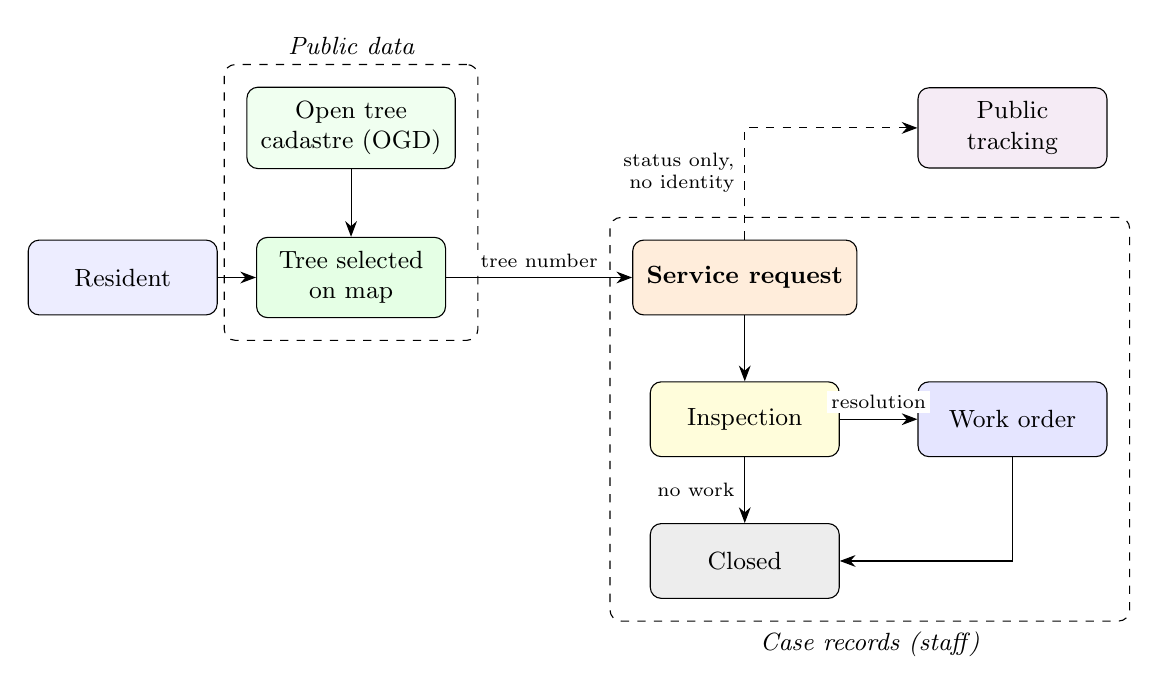
\begin{tikzpicture}[
    box/.style={draw, rounded corners, align=center, font=\small, inner sep=5pt, minimum width=2.4cm, minimum height=0.95cm},
    lbl/.style={font=\scriptsize, fill=white, inner sep=1.5pt},
    layer/.style={draw, dashed, inner sep=8pt, rounded corners},
    arr/.style={-{Stealth[length=2mm]}}
]
\node[box, fill=green!6]   (ogd)     at (2.9, 1.9)   {Open tree\\cadastre (OGD)};
\node[box, fill=blue!7]    (citizen) at (0, 0)       {Resident};
\node[box, fill=green!10]  (map)     at (2.9, 0)     {Tree selected\\on map};
\node[box, fill=orange!14] (sr)      at (7.9, 0)     {\textbf{Service request}};
\node[box, fill=yellow!14] (insp)    at (7.9, -1.8)  {Inspection};
\node[box, fill=blue!10]   (wo)      at (11.3, -1.8) {Work order};
\node[box, fill=gray!14]   (closed)  at (7.9, -3.6)  {Closed};
\node[box, fill=violet!8]  (track)   at (11.3, 1.9)  {Public\\tracking};
\draw[arr] (citizen) -- (map);
\draw[arr] (ogd) -- (map);
\draw[arr] (map) -- node[lbl, above=2pt] {tree number} (sr);
\draw[arr] (sr) -- (insp);
\draw[arr] (insp) -- node[lbl, above=2pt] {resolution} (wo);
\draw[arr] (insp) -- node[lbl, left=2pt] {no work} (closed);
\draw[arr] (wo) |- (closed);
\draw[arr, dashed] (sr.north) |- node[lbl, pos=0.3, left=2pt, align=right] {status only,\\ no identity} (track.west);
\begin{scope}[on background layer]
\node[layer, fit=(ogd)(map), label={[font=\small\itshape]above:Public data}] {};
\node[layer, fit=(sr)(insp)(wo)(closed), label={[font=\small\itshape]below:Case records (staff)}] {};
\end{scope}
\end{tikzpicture}
\caption{SR-centred flow. The resident selects a tree from the open cadastre; the report carries its tree number into one service request that moves through inspection and, if needed, a work order to closure. The public tracking view shows progress but never the reporter's identity.}
\label{fig:model}
\end{figure}

\subsection{Design principles}
\label{sec:principles}

Five principles guided the design. P2 and P3 follow civic-reporting practice \cite{fms,govuk}; P4 and P5 follow case-management practice and privacy by design.

\begin{description}[leftmargin=1.8em,style=nextline]
  \item[P1 — The case is the anchor.] One SR number from intake to closure; inspections and work orders are its steps.
  \item[P2 — Location first, anchored to the tree.] The resident starts on the map and selects an inventoried tree; the report stores its tree number and cadastre attributes, not a free-text location.
  \item[P3 — One thing at a time.] Tree, issue, contact and review are separate steps; the category comes before personal details; the resident checks the answers before sending and receives a reference number with an explanation of what happens next. Open reports on the same tree are shown before a new one is filed.
  \item[P4 — Progress is public, identity is not.] Anyone holding the reference number can follow the case; names, e-mail addresses, phone numbers and staff-internal notes are visible to signed-in staff only.
  \item[P5 — One status language.] The same four phases and colours appear on map pins, in the staff queue and on the tracking page.
\end{description}

%======================================================================
\section{Method}
\label{sec:method}

\subsection{Design science approach}

The study follows design-science research, in which knowledge is produced by building and evaluating an artifact \cite{hevner2004,peffers2007}. The artifact (\S\ref{sec:artifact}) instantiates the case model and principles. It is evaluated in two ways: analytically, with a city-wide analysis of location ambiguity (RQ2), and by verification, with automated tests of its privacy and workflow rules and systematic interface checks (RQ1, RQ3). The study does not include a user study with residents or staff.

\subsection{Data}

Two open datasets of the City of Zürich were retrieved through its WFS services on 20~November~2026 (SHA-256 checksums are archived with the analysis code):

\begin{itemize}
  \item \textbf{Baumkataster} (layer \texttt{baumkataster\_baumstandorte}) \cite{zh-baum}: 81{,}403 trees with tree number, species, planting year, street name and point position; 23{,}177 are classified as street trees (\emph{Strassenbaum}) and 58{,}226 as park and other trees (\emph{Parkbaum}).
  \item \textbf{Adressen Stadt Zürich} (layer \texttt{adrstzh\_adressen\_stzh\_p}) \cite{zh-adr}: 59{,}330 official building addresses, each with the position of its house number.
\end{itemize}

Positions were projected to a local metric plane (equirectangular about the city centre; distortion below 0.1\,\% within the city). Neighbour queries used $k$-d trees.

\subsection{Intake methods compared}

For every tree $t$, I count the \emph{candidate trees} a report about $t$ leaves to be disambiguated:

\begin{itemize}
  \item \textbf{Street name only}: all trees whose recorded street equals that of $t$.
  \item \textbf{Building address}: a resident describing $t$ by an address is modelled as naming the official address nearest to $t$; the candidates are all trees whose nearest address is the same. Trees farther than 60\,m from any address are reported separately, since no address plausibly describes them.
  \item \textbf{Map selection}: all trees within the selection radius $r$ of the tapped point; with an exact tap, the tapped point is the position of $t$.
\end{itemize}

A tree is \emph{uniquely identified} when exactly one candidate remains and it is $t$.

\subsection{Touch error and selection rules}

A tap rarely lands exactly on the tree. Perceived-input offsets of a few millimetres \cite{holz2010,parhi2006} correspond to roughly 2.5--5\,m on the ground at zoom level 19, where trees become selectable in the application (about 0.2\,m per screen pixel at Zürich's latitude), and to twice that at zoom 18. I therefore simulate tap errors of 0, 3, 5 and 8\,m in a uniformly random direction (fixed random seed) for every tree and compare four selection rules:

\begin{itemize}
  \item \textbf{List 5\,m} and \textbf{list 10\,m}: offer all trees within $r$, ordered by distance; the resident chooses.
  \item \textbf{Nearest 10\,m}: select the nearest tree within 10\,m automatically.
  \item \textbf{Hybrid 10\,m}: select the nearest tree automatically unless the second-nearest is within 1.5 times its distance, in which case offer a short list.
\end{itemize}

For each rule I record whether the intended tree is offered (as the single result or in the list), whether it is found in one step, and whether a single \emph{wrong} tree is returned. The last outcome is the costly one: the report would be attached to another tree without anyone noticing.

\subsection{Verification and ethics}

The artifact's privacy, validation and authentication rules are covered by 18 automated tests, including in-process API tests (\S\ref{sec:privacy}). The interface was checked automatically at five screen sizes (360\,px to 1366\,px wide, portrait and landscape) in ten interaction states for overlapping controls, hidden controls, horizontal overflow and touch-target size. All case data used in the demonstrator are fictional: fourteen requests on real trees with invented names and \texttt{example.ch} addresses, created through the application's own workflow. No data from residents or from municipal systems were used.

%======================================================================
\section{The demonstrator}
\label{sec:artifact}

The \appname{} application is a working prototype of the case model, not a production system. It reads trees from the City of Zürich open-data services and stores cases in its own database. The interface is available in English and German and adapts from phones to desktop screens.

\subsection{Resident path}

A resident starts from the map and chooses \emph{Report a tree issue}, optionally centring the map on their position. Selecting a tree opens its card with species, tree number, planting year and crown diameter (Figure~\ref{fig:tree}). The report then takes four steps (Figure~\ref{fig:report}): the tree and its location, the issue (nine categories; for hazards the form advises calling the emergency services first), contact details, and a review in which every answer can be changed. Before the issue step, open requests already filed for the same tree are listed. On submission the resident receives the SR number and a short explanation of the next steps (Figure~\ref{fig:phone}).

\begin{figure}[htbp]
\centering
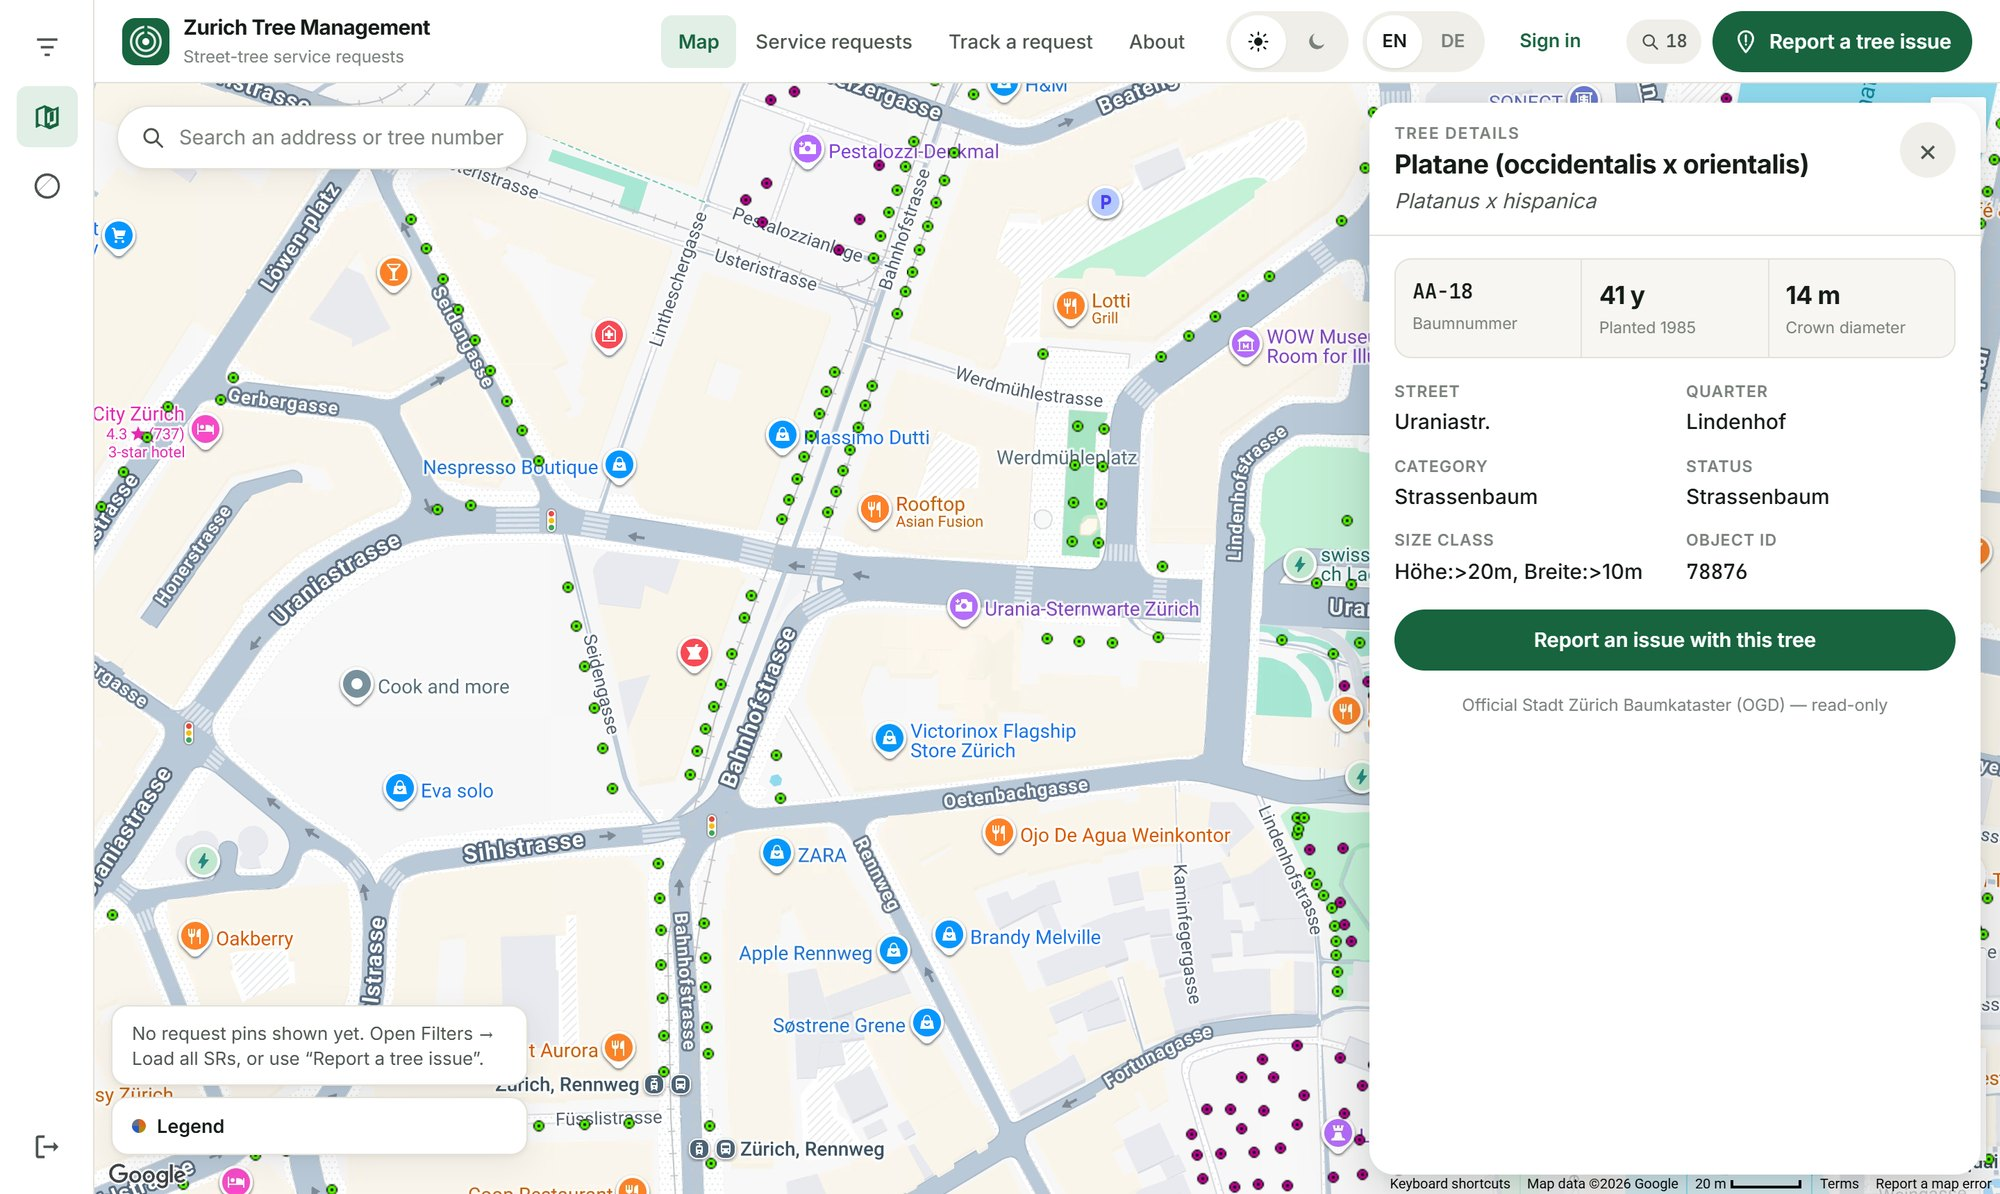
\includegraphics[width=\linewidth]{fig-tree-card.jpg}
\caption{Tree card. Selecting a tree on the map shows its cadastre record---here a plane tree planted in 1985---and offers to report an issue with exactly this tree.}
\label{fig:tree}
\end{figure}

\begin{figure}[htbp]
\centering
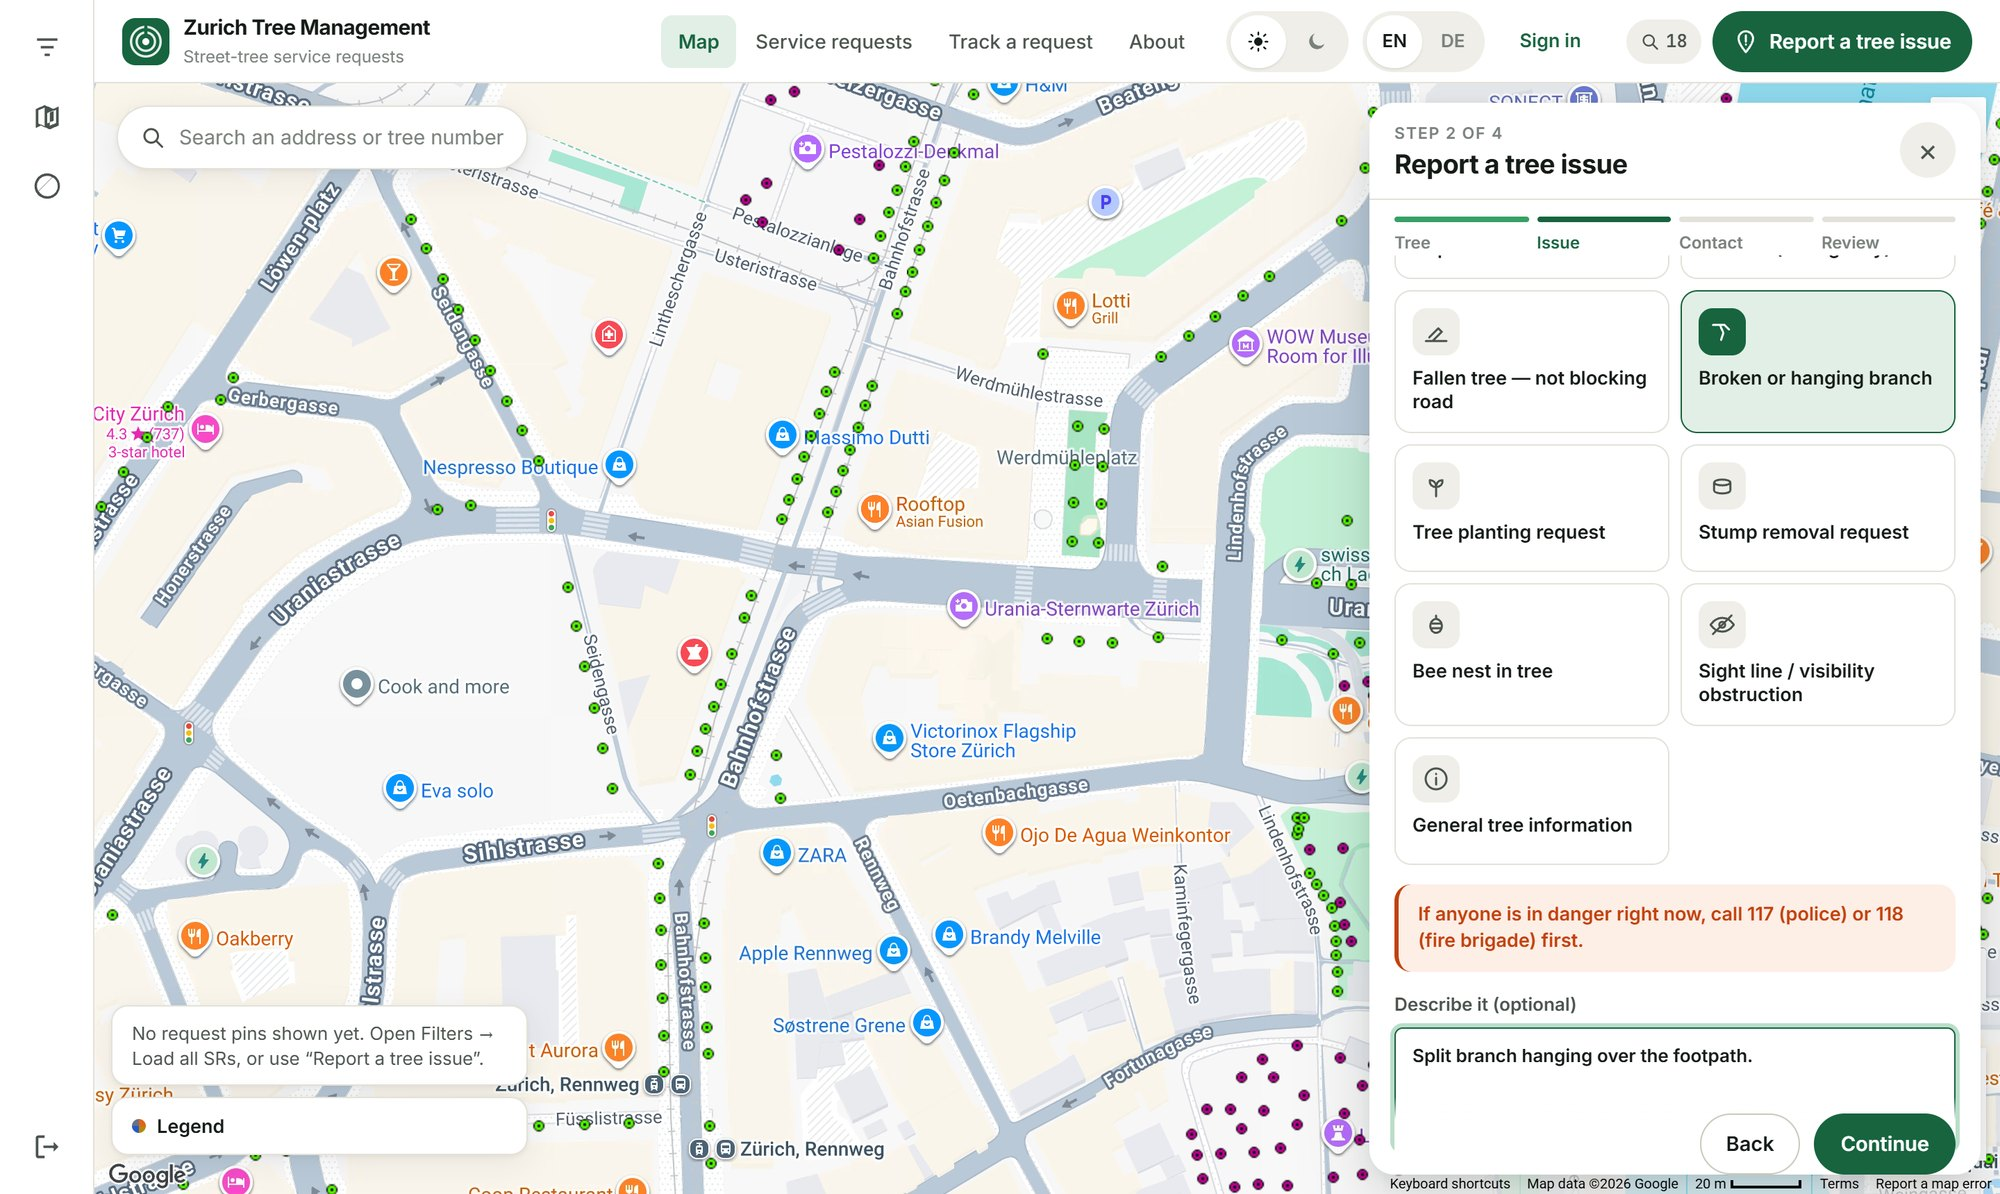
\includegraphics[width=\linewidth]{fig-report-issue.jpg}
\caption{Second of four reporting steps. Issue categories are shown as cards; for hazardous situations the form points to the emergency numbers before continuing.}
\label{fig:report}
\end{figure}

\begin{figure}[htbp]
\centering
\begin{subfigure}[t]{0.42\linewidth}\centering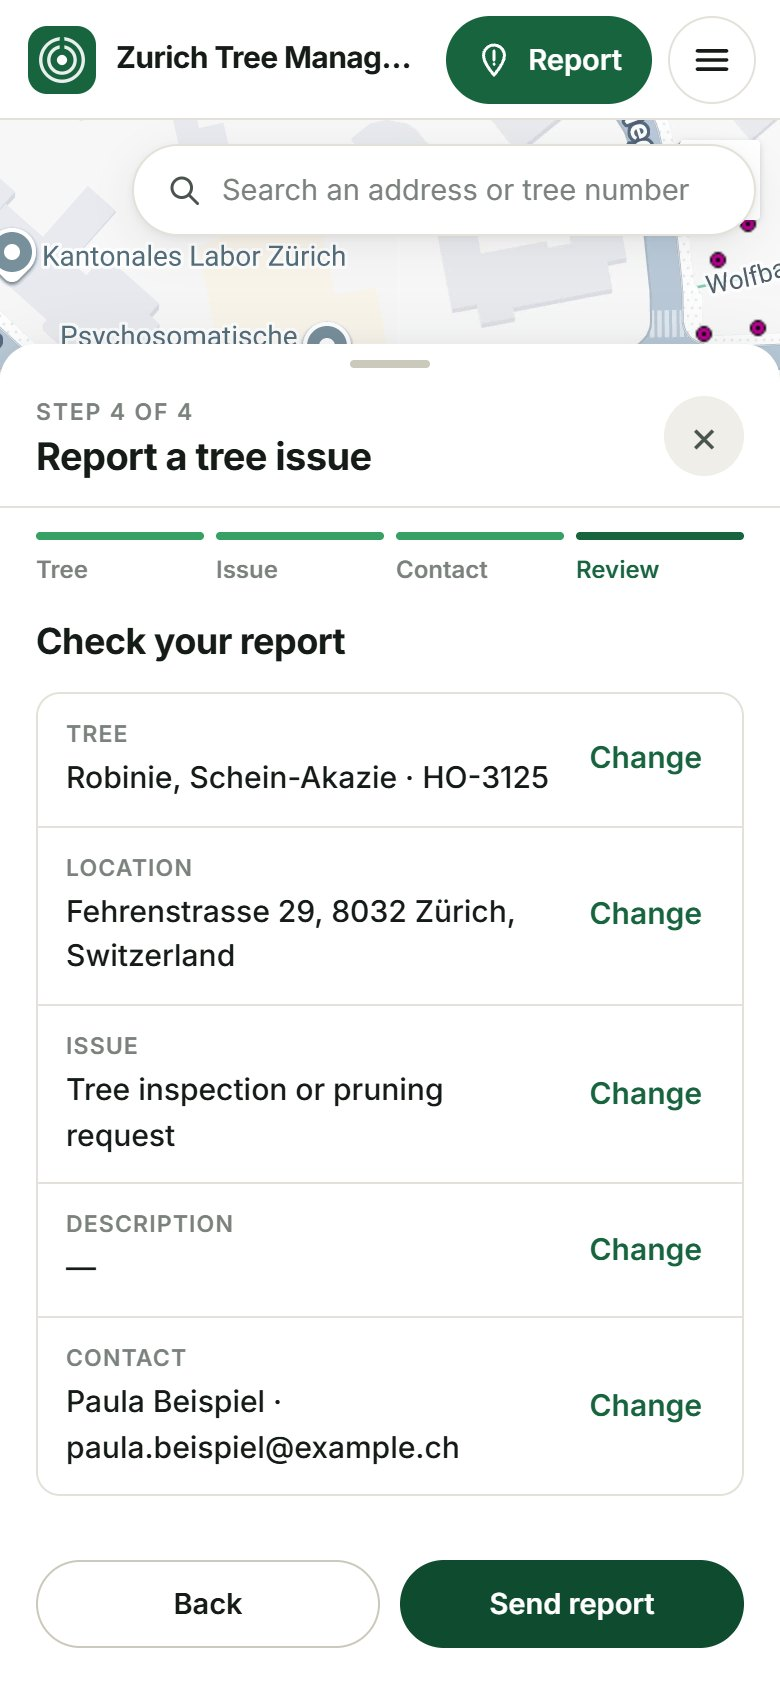
\includegraphics[width=\linewidth]{fig-phone-review.jpg}\caption{Review before sending.}\end{subfigure}\hspace{0.04\linewidth}%
\begin{subfigure}[t]{0.42\linewidth}\centering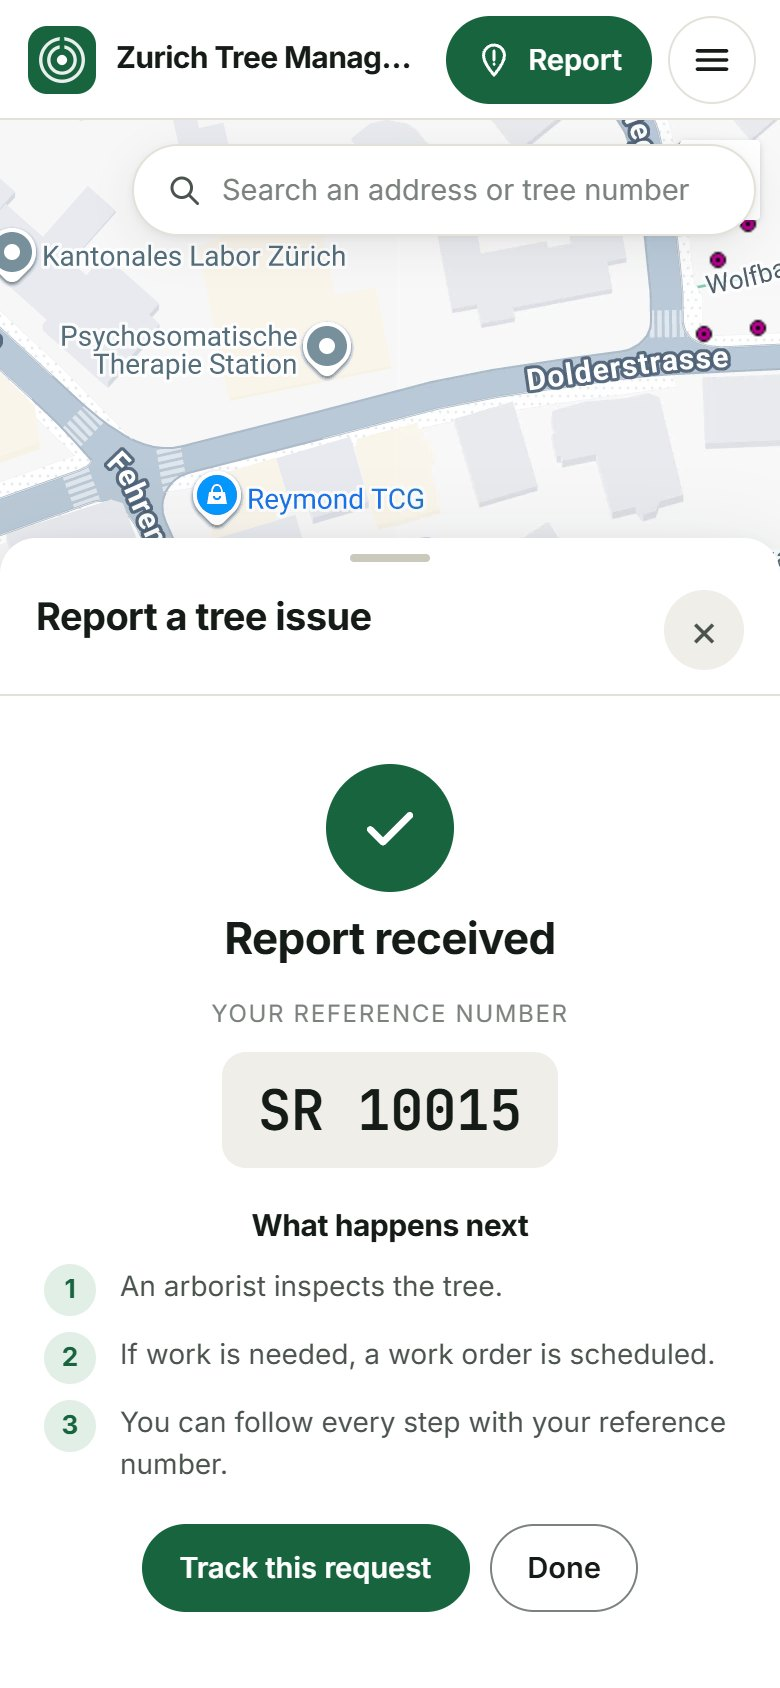
\includegraphics[width=\linewidth]{fig-phone-confirmation.jpg}\caption{Confirmation with reference number.}\end{subfigure}
\caption{The last reporting step and the confirmation on a phone.}
\label{fig:phone}
\end{figure}

With the reference number, anyone can open the public tracking page (Figure~\ref{fig:tracking}). It shows the request type, the tree, the street, the four phases and a dated timeline---and, by design, nothing about who filed the request.

\begin{figure}[htbp]
\centering
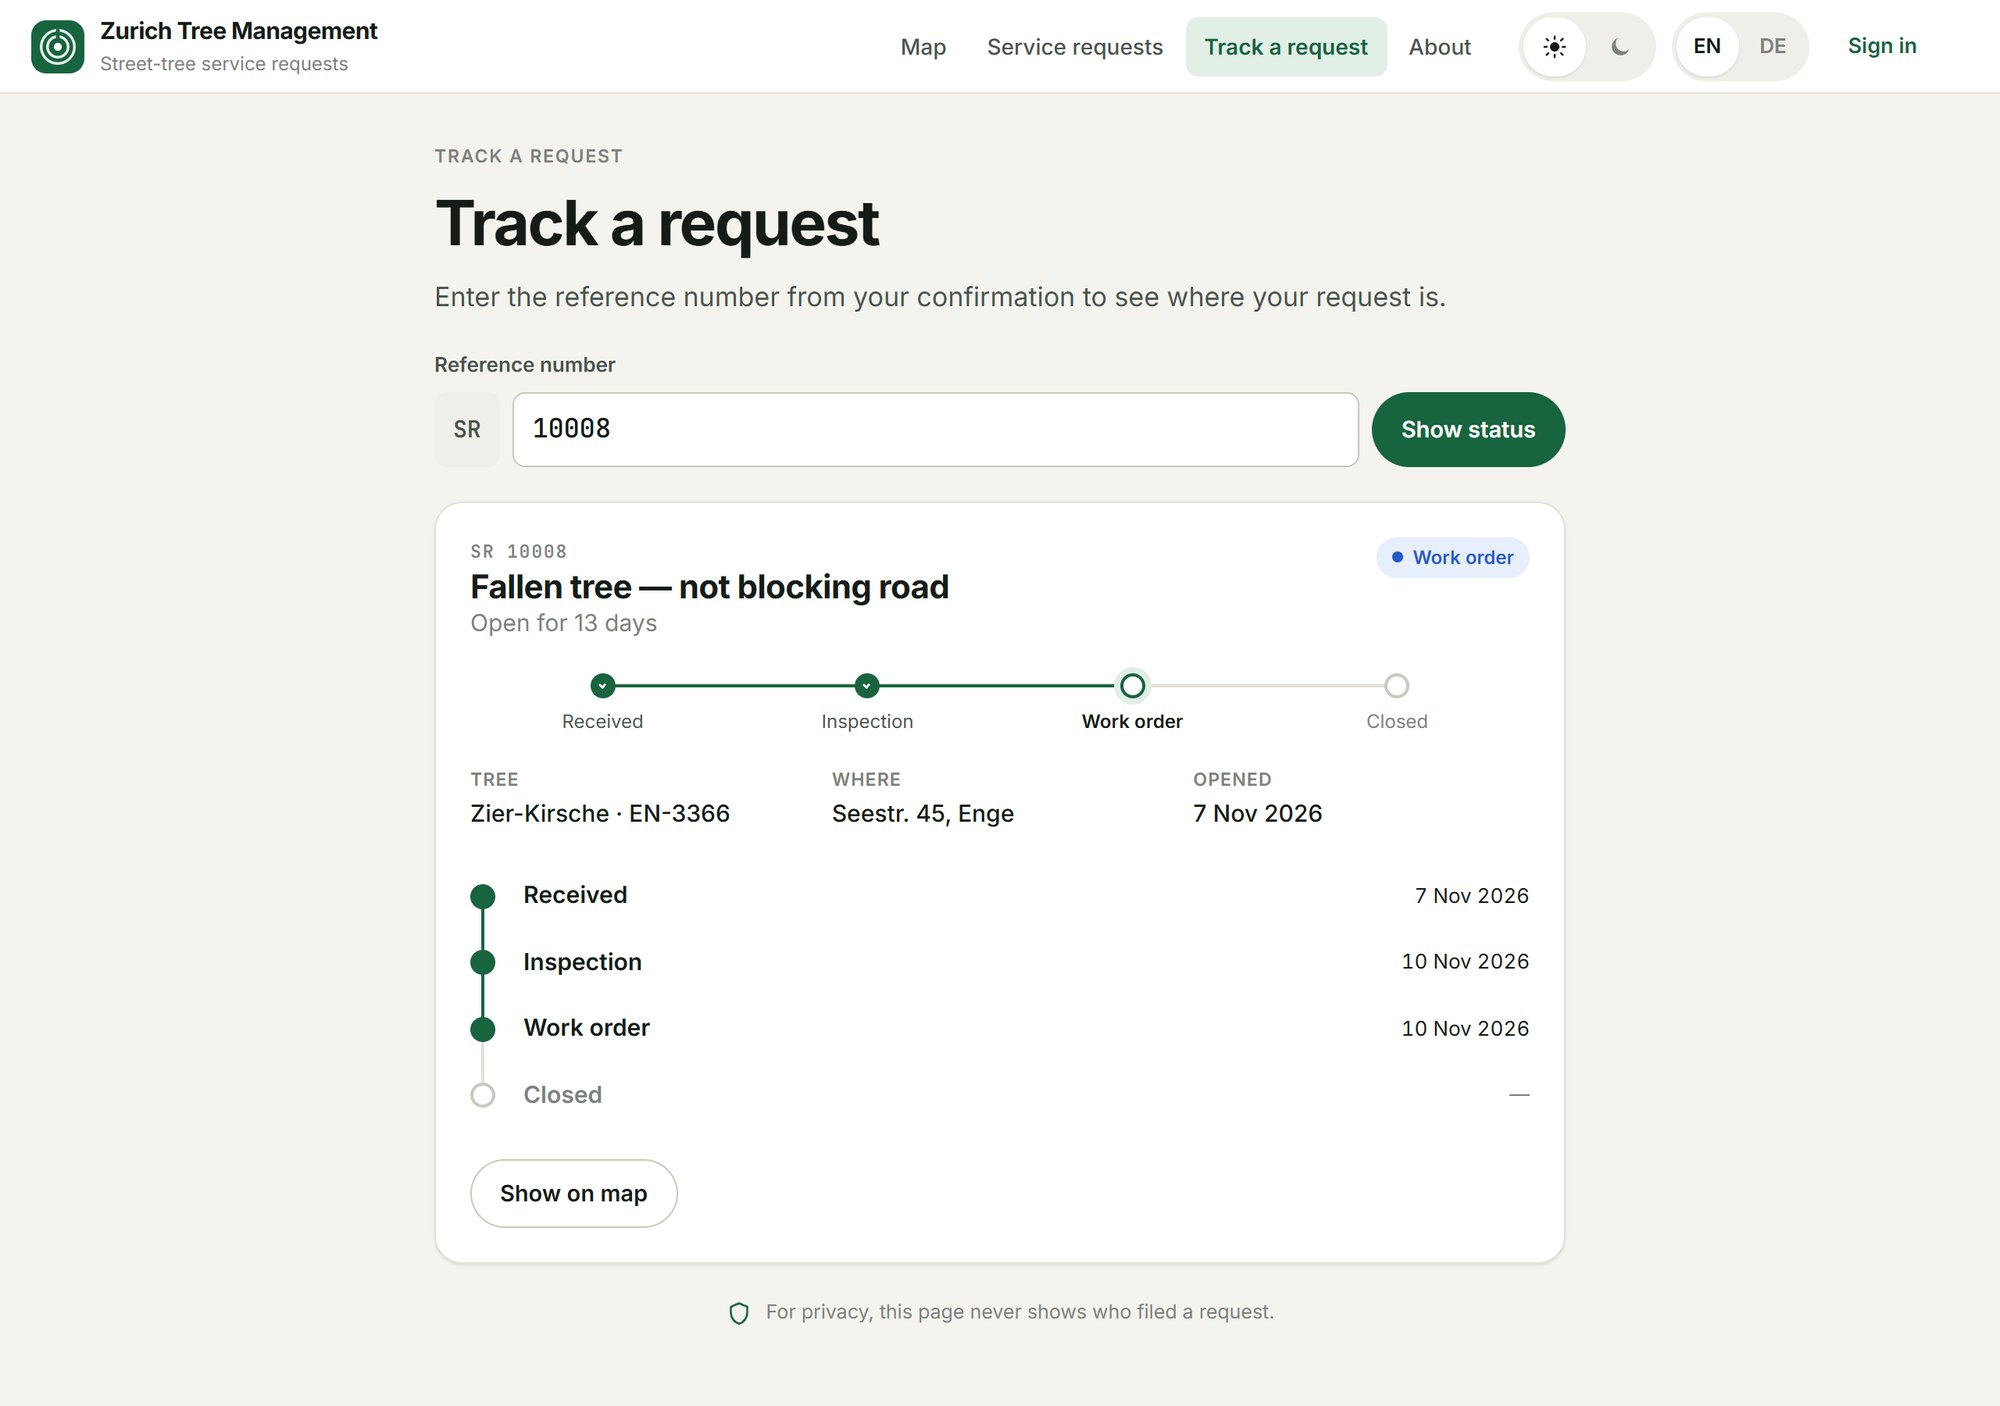
\includegraphics[width=0.86\linewidth]{fig-tracking.jpg}
\caption{Public tracking page for a request in the work-order phase. The page is driven by the same phase logic as the staff views and contains no personal data.}
\label{fig:tracking}
\end{figure}

\subsection{Staff path}

Signed-in staff see request pins on the map, coloured by phase (Figure~\ref{fig:map}), and a desk that lists all requests with their age and an overview of the queue: open, urgent, in inspection, with work orders, closed, and the age of the oldest open request (Figure~\ref{fig:desk}). Each case opens with its phase bar and key facts at the top, followed by tabs for details, inspection, work order and activities (Figure~\ref{fig:desk-insp}). Inspection and work-order transitions enforce the rules in Table~\ref{tab:phase}.

\begin{figure}[htbp]
\centering
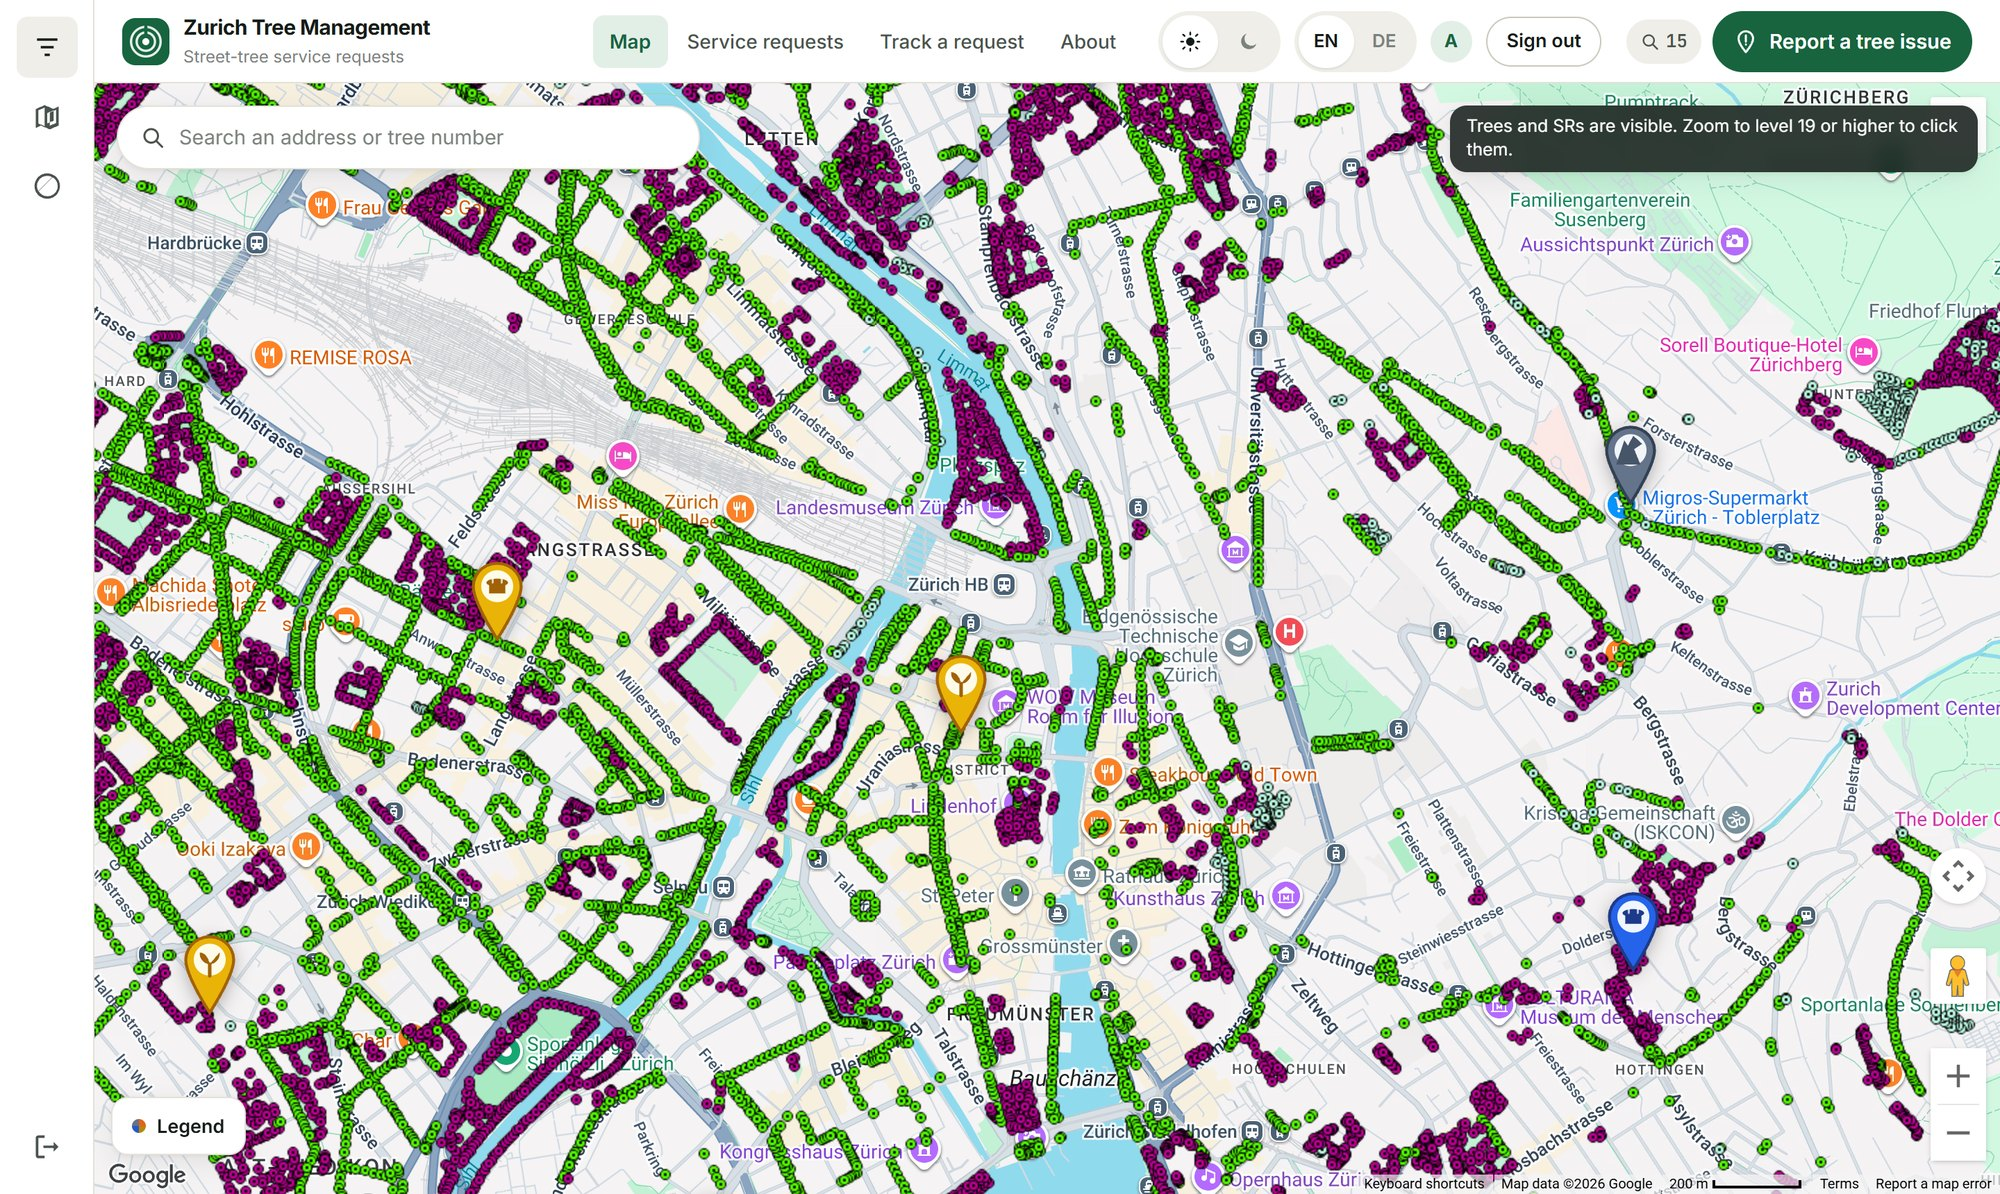
\includegraphics[width=\linewidth]{fig-map-overview.jpg}
\caption{Staff map. Request pins are coloured by phase (received, inspection, work order, closed) over the official tree layer.}
\label{fig:map}
\end{figure}

\begin{figure}[htbp]
\centering
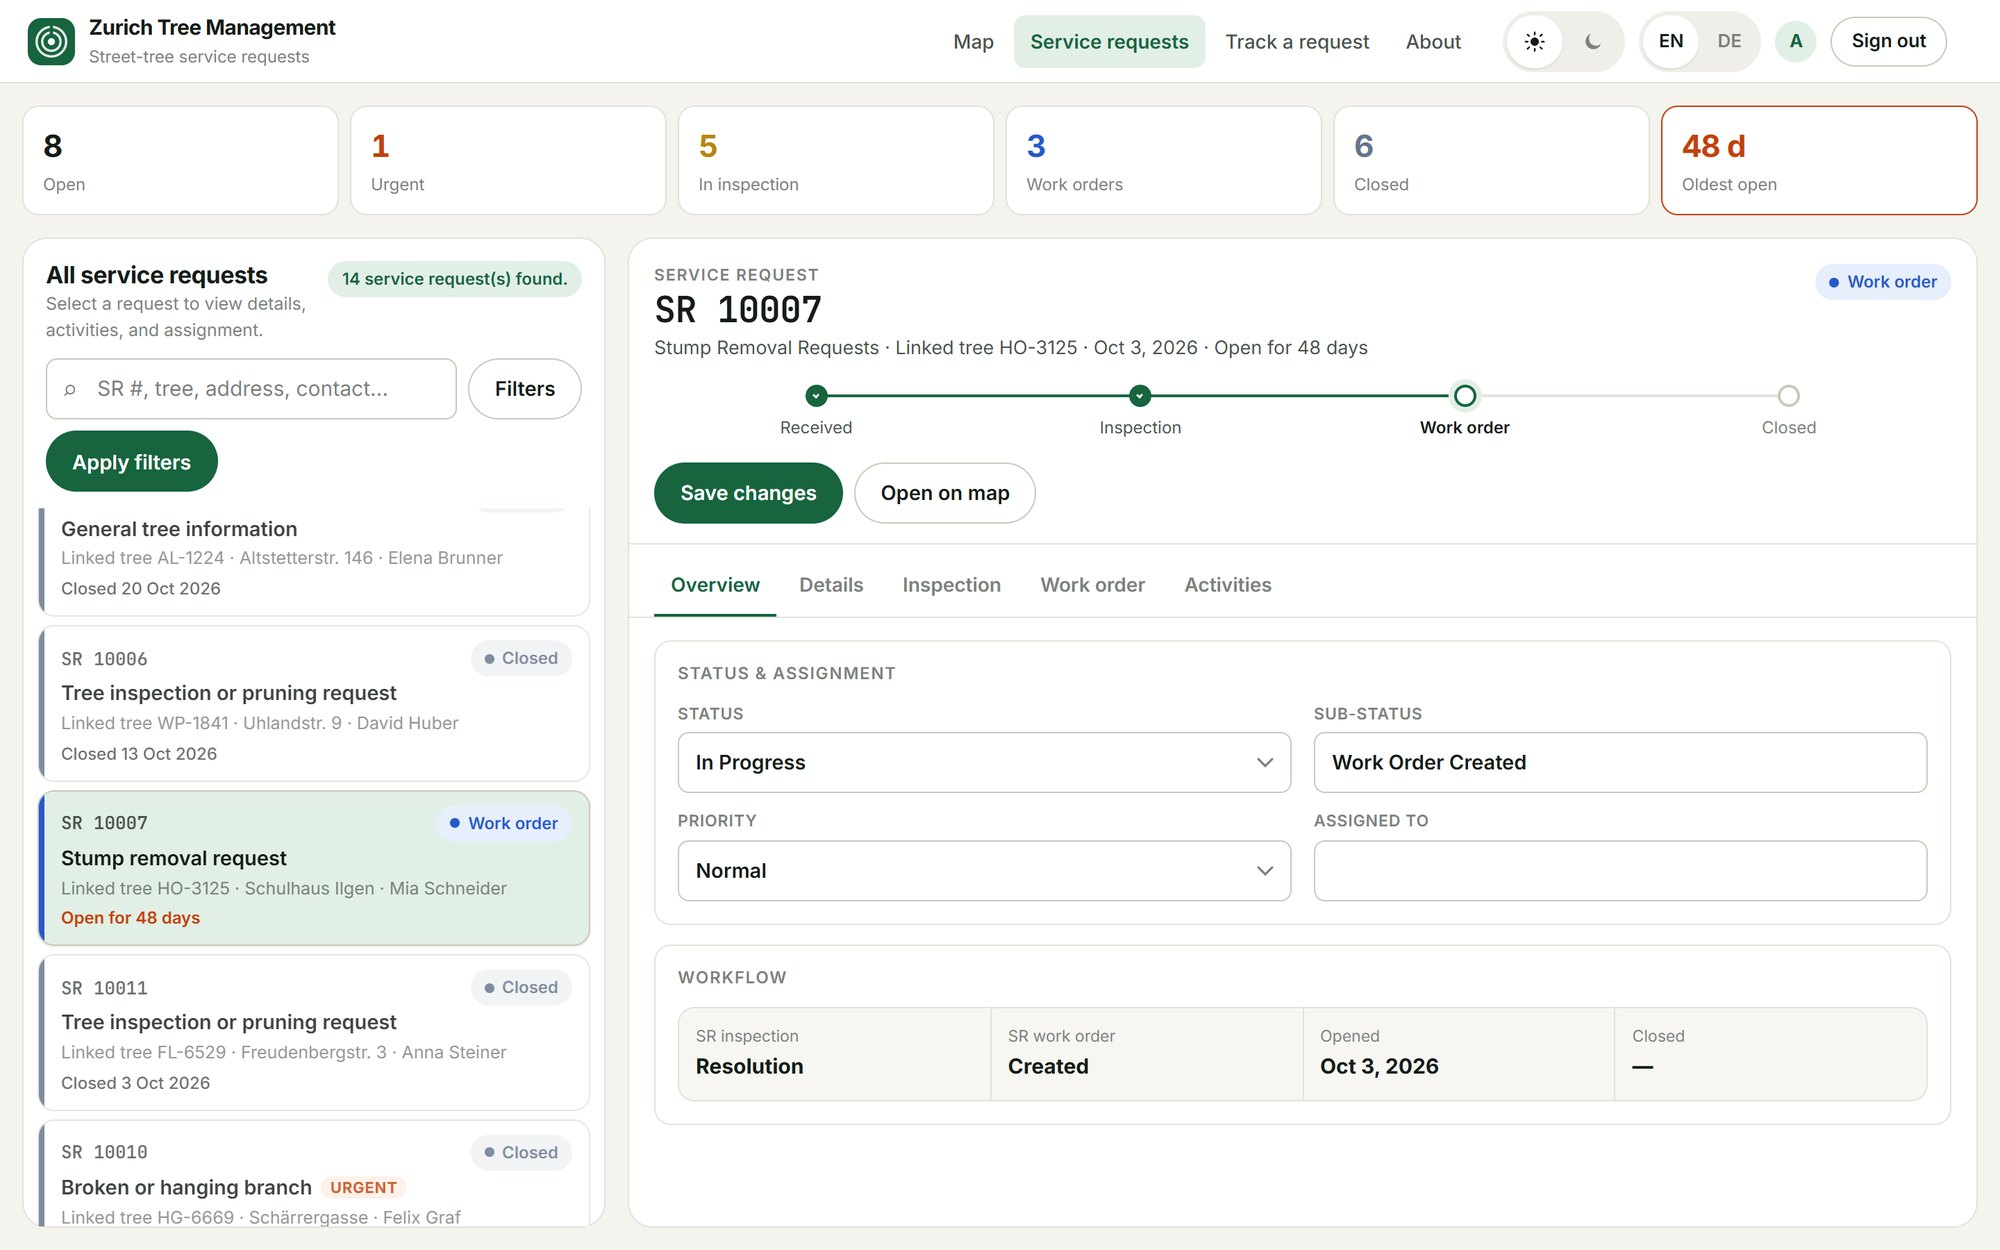
\includegraphics[width=\linewidth]{fig-desk.jpg}
\caption{Staff desk. The queue overview and the age of each request make urgency and backlog visible; the selected case shows its phase bar above the record.}
\label{fig:desk}
\end{figure}

\begin{figure}[htbp]
\centering
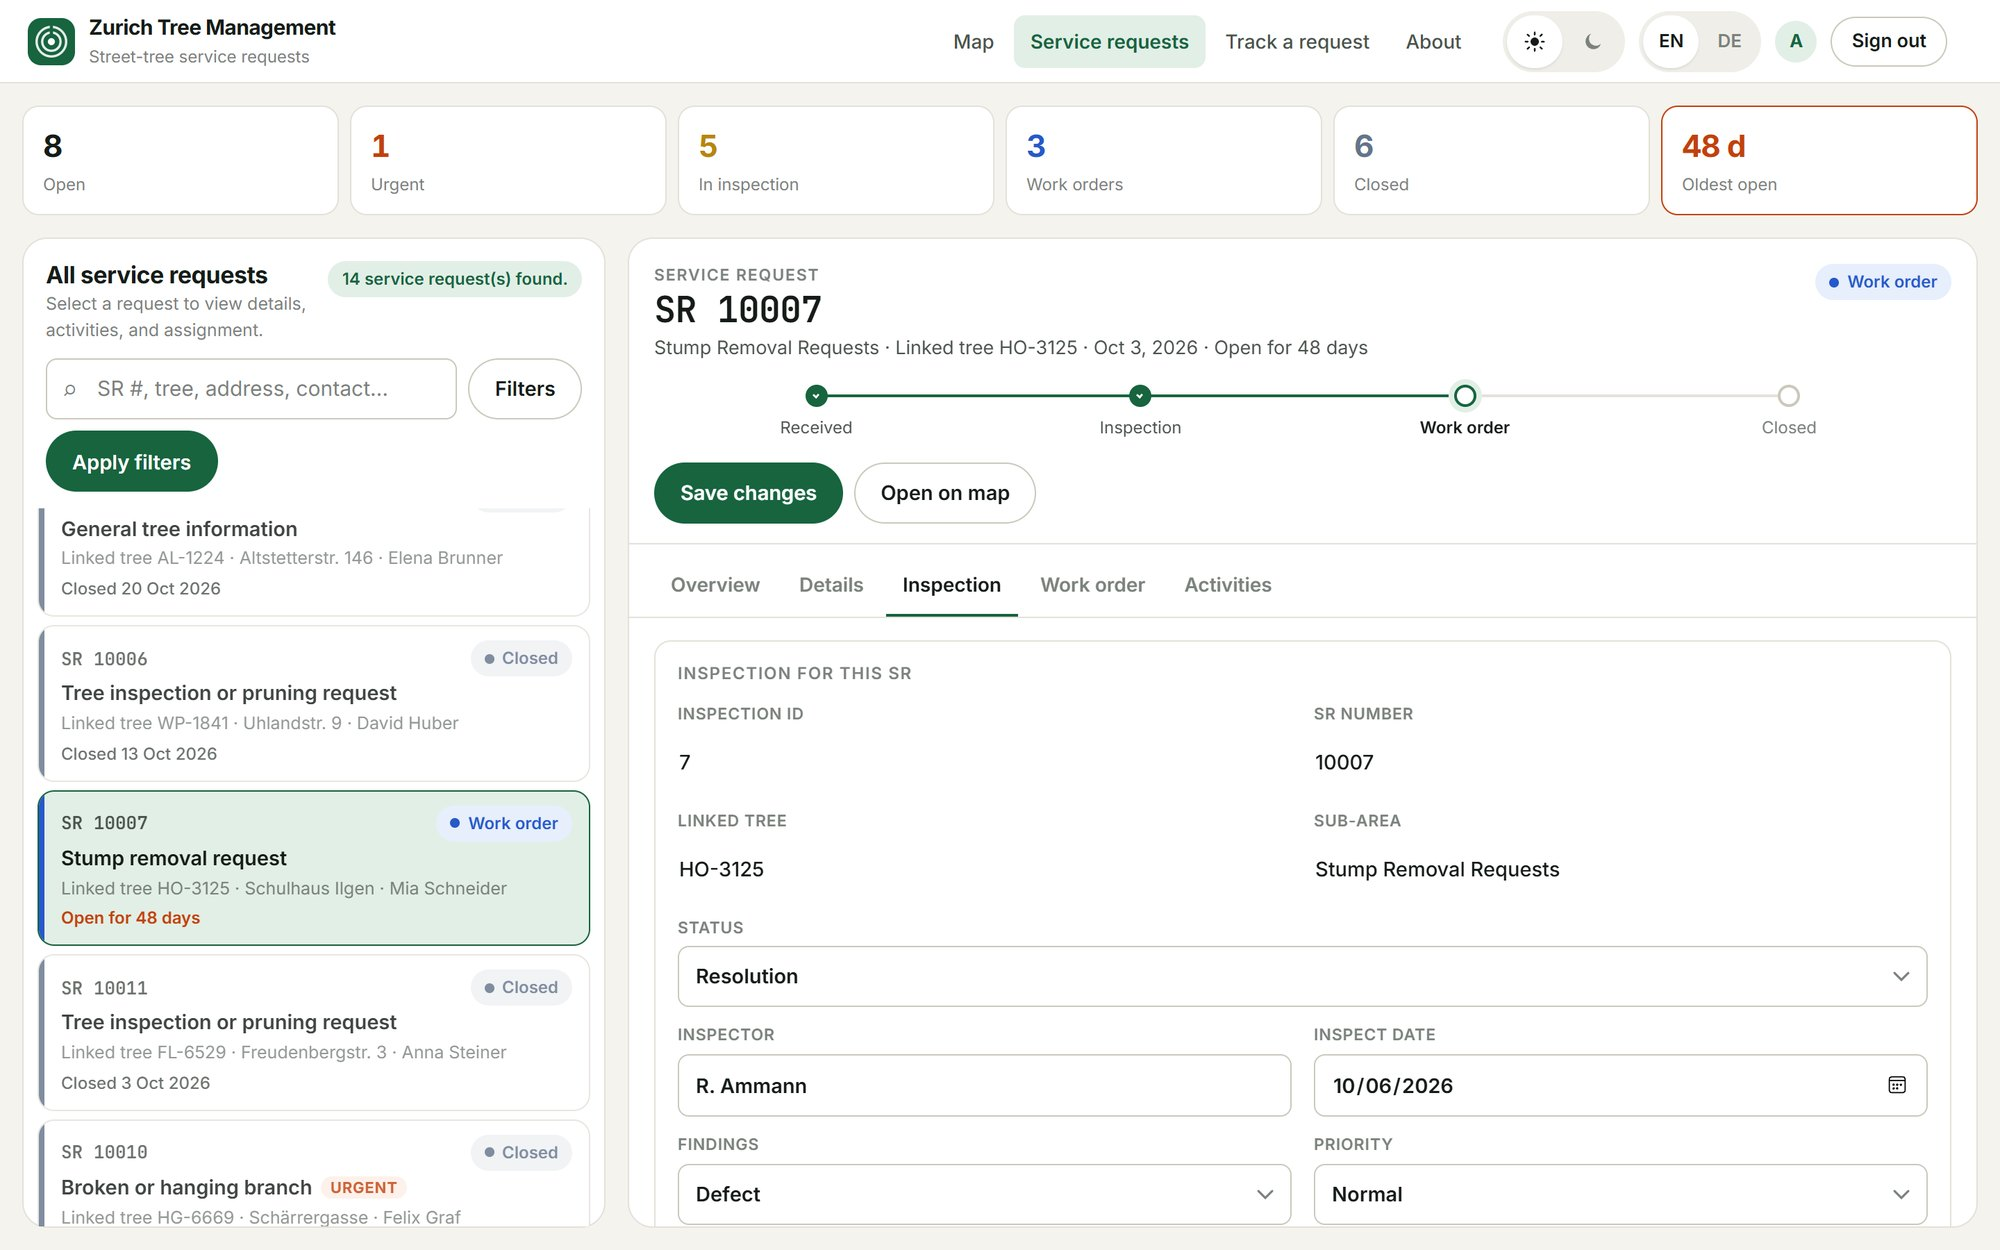
\includegraphics[width=\linewidth]{fig-desk-inspection.jpg}
\caption{Inspection of a case. Closing an inspection with \emph{Resolution} requires a work-order type and a comment and issues a work order under the same SR.}
\label{fig:desk-insp}
\end{figure}

\subsection{Implementation}

The application is built with ASP.NET Core~8 (Razor Pages and a JSON API), Entity Framework Core and SQL Server. The map uses the Google Maps JavaScript API with the Zürich tree layer served through the city's WMS; tree look-ups query the WFS and convert between WGS84 and the Swiss LV95 reference system. Creating a request also creates its inspection in one transaction, so no case exists without its first workflow step. The selection radius is configurable (default 10\,m, \S\ref{sec:pick}). Source code, database scripts, the fictional demo data and the analysis code are published under an open licence (see \emph{Data and code}).

%======================================================================
\section{Privacy and security}
\label{sec:privacy}

Combining a public map with case records creates an obvious risk: request records contain the reporter's name, e-mail address and phone number, and staff add internal notes. Principle P4 is enforced in the server's API rather than in the interface, so that no client---map, tracking page or a direct API call---can obtain more than its viewer may see:

\begin{itemize}
  \item \textbf{Redaction at the API boundary.} Every endpoint that returns case data passes it through one redaction step. For anonymous viewers, contact fields and internal notes on inspections, work orders and activities are removed, and records are flagged so the interface can explain why they are hidden.
  \item \textbf{No inference through search.} Anonymous search does not match contact fields, so it cannot reveal whether a given person filed a request.
  \item \textbf{Validation of anonymous input.} A report is accepted only if its location lies within the city and its category is one of the offered request types; field lengths are bounded.
  \item \textbf{Abuse limits.} Reports and sign-in attempts are rate-limited per network address.
  \item \textbf{Authentication.} The demonstrator's demo sign-in is disabled unless explicitly enabled in a development configuration, and credentials are compared in constant time.
\end{itemize}

These properties are covered by automated tests: unit tests of the redaction for anonymous and signed-in viewers, and in-process API tests showing that out-of-area locations and unknown categories are rejected, that repeated reports are throttled, and that editing requires sign-in. A public privacy notice states what is stored, who can see it and where it is processed.

%======================================================================
\section{Results}
\label{sec:results}

\subsection{Location ambiguity by intake method}

Table~\ref{tab:intake} shows the number of candidate trees each intake method leaves. A street name alone is of little use: half of all trees stand on a street with 47 or more recorded trees. A building address narrows the search but rarely identifies one tree: for street trees, the median address leaves three candidates and identifies a single tree in 14.0\,\% of cases; for park trees the median is 13 candidates and the share is 3.4\,\%. The median distance from a tree to its nearest address is 24.6\,m (90th percentile 72.7\,m), and 14.8\,\% of all trees lie more than 60\,m from any address and cannot be described by one at all.

\begin{table}[htbp]
\centering
\caption{Candidate trees left by each intake method. Map selection uses the application's 10\,m list with an exact tap; the address method excludes trees more than 60\,m from any address.}
\label{tab:intake}
\begin{tabular}{@{}llrrrr@{}}
\toprule
\textbf{Trees} & \textbf{Intake method} & \textbf{Median} & \textbf{90th pct.} & \textbf{Unique} & \textbf{$\geq$5 cand.} \\
\midrule
Street trees  & Street name only  & 5  & 78  & 11.4\,\% & 51.8\,\% \\
($n=23{,}177$) & Building address & 3  & 13  & 14.0\,\% & 35.3\,\% \\
              & Map selection     & 2  & 4   & 25.3\,\% & 7.3\,\% \\
\addlinespace
Park \& other & Street name only  & 86 & 965 & 3.4\,\%  & 92.8\,\% \\
($n=58{,}226$) & Building address & 13 & 65  & 3.4\,\%  & 81.6\,\% \\
              & Map selection     & 3  & 9   & 14.4\,\% & 33.5\,\% \\
\bottomrule
\end{tabular}
\end{table}

Map selection also leaves more than one candidate in most cases, because trees stand close together. The difference lies in \emph{who} resolves the ambiguity and \emph{when}. With an address, candidates are unlabelled and the question of which tree was meant is left to staff, often on site. With map selection, the resident sees a short list of labelled trees---species, tree number and distance---while still at the location, and confirms one; the stored report then refers to exactly one tree number.

\subsection{Selection rules under touch error}
\label{sec:pick}

Table~\ref{tab:pick} compares the four selection rules for street trees. A 5\,m list works for precise taps but fails once the error reaches the radius: at a 5\,m error, the intended tree is offered in only 50.0\,\% of taps and a wrong single tree is returned in 11.1\,\%. Automatic nearest-tree selection always finds the tree with a perfect tap but degrades quickly, returning a wrong tree in 25.5\,\% of street-tree taps at 5\,m and 58.3\,\% at 8\,m. The hybrid rule sits between the two. The 10\,m list keeps the intended tree among the choices in 99.8\,\% of street-tree taps even at 8\,m (97.1\,\% for all trees) and never returns a single wrong tree; its cost is that a list (mean 2.8 trees) must be confirmed in about three of four selections.

\begin{table}[htbp]
\centering
\caption{Selection rules under simulated touch error (street trees, $n=23{,}177$). \emph{Offered}: intended tree is the single result or in the list. \emph{Wrong}: a single, wrong tree is returned.}
\label{tab:pick}
\begin{tabular}{@{}lrrrrrrrr@{}}
\toprule
& \multicolumn{4}{c}{\textbf{Intended tree offered}} & \multicolumn{4}{c}{\textbf{Wrong single tree}} \\
\cmidrule(lr){2-5}\cmidrule(lr){6-9}
\textbf{Rule} & 0\,m & 3\,m & 5\,m & 8\,m & 0\,m & 3\,m & 5\,m & 8\,m \\
\midrule
List 5\,m     & 100.0 & 100.0 & 50.0 & 0.0  & 0.0 & 0.0 & 11.1 & 29.6 \\
List 10\,m    & 100.0 & 100.0 & 99.9 & 99.8 & 0.0 & 0.0 & 0.0  & 0.0 \\
Nearest 10\,m & 100.0 & 94.7  & 74.5 & 41.7 & 0.0 & 5.3 & 25.5 & 58.3 \\
Hybrid 10\,m  & 100.0 & 98.2  & 91.8 & 66.4 & 0.0 & 1.5 & 6.8  & 27.9 \\
\bottomrule
\end{tabular}
\end{table}

Because a report attached to the wrong tree sends an arborist to the wrong place and may never be noticed, the application uses the 10\,m list ordered by distance. The extra confirming tap coincides with the first reporting step, which already asks ``Is this the right tree?''.

%======================================================================
\section{Discussion}
\label{sec:discussion}

\paragraph{RQ1 — one traceable case.}
Treating the SR as the case and deriving its phase from the state of its inspection and work order gives residents and staff the same view of progress. Because the phase is computed rather than entered, the map, the staff queue and the tracking page cannot disagree. Requiring a comment at each closing transition leaves a written trace of every decision. One limitation is that the model assumes one tree per request: a storm that damages a whole row produces many separate requests, and an incident record grouping several SRs would represent such events better.

\paragraph{RQ2 — location ambiguity.}
The analysis supports anchoring reports to inventoried trees. Addresses identify a single tree only rarely, and for park trees almost never. Tree-anchored intake does not make selection unambiguous by itself---trees are dense---but it moves disambiguation to the moment and place where it is easiest, and it produces a report linked to one tree number. The selection-rule comparison adds a concrete design lesson: the selection radius must be chosen against realistic touch error, and an explicit choice is safer than automatic selection. These findings concern \emph{geometric} ambiguity; whether residents choose correctly from the list, and how much staff time this saves, are questions for a field study.

\paragraph{RQ3 — privacy.}
Public status and private identity can coexist if redaction is enforced once, at the boundary where case data leave the server. Doing it in the interface alone would leave the data exposed to anyone calling the API directly. The same reasoning applies to search, which must not become a way to test whether a person has reported something.

\paragraph{Relation to practice.}
Enterprise asset-management suites integrate maps, cases and work orders, but their workflows can be hard to explain to non-specialists. A small, inspectable implementation of the same ideas is useful as a reference for design discussions, teaching and comparison, even though it is not intended for production use.

\paragraph{Limitations.}
The study has no user study: usability, the accuracy of residents' choices and staff efficiency were not measured. The address method models a resident as naming the nearest building address, which simplifies how people describe places; landmarks and descriptions such as ``opposite the school'' are not modelled. Touch error is simulated with a single error distance per run and a uniform direction rather than measured on devices. The analysis and the request categories are specific to Zürich. The demonstrator's authentication is a demonstration mechanism and has not been assessed for internet-facing operation.

%======================================================================
\section{Conclusion}
\label{sec:conclusion}

This paper set out to show how tree-related service requests can be organised around one case anchored to one tree, and to quantify what that anchoring gains. The case model and its implementation keep intake, inspection, work order and closure in one record, show residents the same progress as staff, and keep identities private by enforcing redaction in the API. The city-wide analysis shows that address descriptions rarely identify a tree in Zürich, while map selection with an explicit, distance-ordered 10\,m list keeps the intended tree available to the resident under realistic touch error and never attaches a report to the wrong tree silently.

Three directions follow. A field study with residents and arborists should measure selection accuracy and handling time. An incident record should group requests caused by the same event. And the analysis should be repeated in other cities with open tree inventories to test how far the findings generalise.

%======================================================================
\section*{Data and code}

\begin{itemize}
  \item \textbf{Source code, database scripts and fictional demo data:} \url{\repourl}, archived on Zenodo \archivedoi.
  \item \textbf{Analysis:} \texttt{analysis/ambiguity\_analysis.py} and \texttt{analysis/pick\_design.py} in the same repository, with results and the SHA-256 checksums of the input data.
  \item \textbf{Input data:} City of Zürich open data, \emph{Baumkataster} \cite{zh-baum} and \emph{Adressen Stadt Zürich} \cite{zh-adr}, retrieved via WFS on 20~November~2026.
\end{itemize}

%======================================================================
\begin{thebibliography}{99}
\small

\bibitem{batty2018} M.~Batty, ``Digital twins,'' \emph{Environment and Planning B: Urban Analytics and City Science}, vol.~45, no.~5, pp.~817--820, 2018.

\bibitem{beatley2011} T.~Beatley, \emph{Biophilic Cities: Integrating Nature into Urban Design and Planning}. Washington, DC: Island Press, 2011.

\bibitem{cavoukian2009} A.~Cavoukian, \emph{Privacy by Design: The 7 Foundational Principles}. Toronto: Information and Privacy Commissioner of Ontario, 2009.

\bibitem{clark2013} B.~Y. Clark, J.~L. Brudney, and S.-G. Jang, ``Coproduction of government services and the new information technology: Investigating the distributional biases,'' \emph{Public Administration Review}, vol.~73, no.~5, pp.~687--701, 2013.

\bibitem{escobedo2011} F.~J. Escobedo, T.~Kroeger, and J.~E. Wagner, ``Urban forests and pollution mitigation: Analyzing ecosystem services and disservices,'' \emph{Environmental Pollution}, vol.~159, no.~8--9, pp.~2078--2087, 2011.

\bibitem{fadp} Swiss Confederation, \emph{Federal Act on Data Protection (FADP)}, SR~235.1, revised version in force since 1~September 2023.

\bibitem{fms} mySociety, \emph{FixMyStreet} (open-source reporting platform), \url{https://github.com/mysociety/fixmystreet}.

\bibitem{goodchild2007} M.~F. Goodchild, ``Citizens as sensors: the world of volunteered geography,'' \emph{GeoJournal}, vol.~69, no.~4, pp.~211--221, 2007.

\bibitem{govuk} Government Digital Service, \emph{GOV.UK Design System: Patterns} (question pages, check answers, confirmation pages), \url{https://design-system.service.gov.uk/patterns/}.

\bibitem{hevner2004} A.~R. Hevner, S.~T. March, J.~Park, and S.~Ram, ``Design science in information systems research,'' \emph{MIS Quarterly}, vol.~28, no.~1, pp.~75--105, 2004.

\bibitem{holz2010} C.~Holz and P.~Baudisch, ``The generalized perceived input point model and how to double touch accuracy by extracting fingerprints,'' in \emph{Proc.\ CHI 2010}, pp.~581--590, ACM, 2010.

\bibitem{janssen2012} M.~Janssen, Y.~Charalabidis, and A.~Zuiderwijk, ``Benefits, adoption barriers and myths of open data and open government,'' \emph{Information Systems Management}, vol.~29, no.~4, pp.~258--268, 2012.

\bibitem{minkoff2016} S.~L. Minkoff, ``NYC 311: A tract-level analysis of citizen--government contacting in New York City,'' \emph{Urban Affairs Review}, vol.~52, no.~2, pp.~211--246, 2016.

\bibitem{obrien2018} D.~T. O'Brien, \emph{The Urban Commons: How Data and Technology Can Rebuild Our Communities}. Cambridge, MA: Harvard University Press, 2018.

\bibitem{open311} Open311, \emph{GeoReport v2 specification}, \url{https://www.open311.org}.

\bibitem{parhi2006} P.~Parhi, A.~K. Karlson, and B.~B. Bederson, ``Target size study for one-handed thumb use on small touchscreen devices,'' in \emph{Proc.\ MobileHCI 2006}, pp.~203--210, ACM, 2006.

\bibitem{peffers2007} K.~Peffers, T.~Tuunanen, M.~A. Rothenberger, and S.~Chatterjee, ``A design science research methodology for information systems research,'' \emph{Journal of Management Information Systems}, vol.~24, no.~3, pp.~45--77, 2007.

\bibitem{trist1982} E.~Trist and H.~Murray (eds.), \emph{The Social Engagement of Social Science}, vol.~II: \emph{The Socio-Technical Perspective}. Philadelphia: University of Pennsylvania Press, 1993.

\bibitem{zandbergen2008} P.~A. Zandbergen, ``A comparison of address point, parcel and street geocoding techniques,'' \emph{Computers, Environment and Urban Systems}, vol.~32, no.~3, pp.~214--232, 2008.

\bibitem{zh-adr} Stadt Zürich, \emph{Adressen Stadt Zürich} (open data; WFS layer \texttt{adrstzh\_adressen\_stzh\_p}), \url{https://data.stadt-zuerich.ch/dataset/geo_adressen_stadt_zuerich}.

\bibitem{zh-baum} Stadt Zürich, \emph{Baumkataster} (open data; WFS layer \texttt{baumkataster\_baumstandorte}), \url{https://www.ogd.stadt-zuerich.ch/wfs/geoportal/Baumkataster}.

\bibitem{zwn} mySociety, ``Case study: Züri wie neu,'' \url{https://www.mysociety.org/community/fixmystreet/case-study-zuri-wie-neu/}.

\end{thebibliography}
\end{document}
